\documentclass[a4paper,12pt]{article}

\usepackage{hyperref}
\usepackage{graphicx}
\usepackage[svgnames, table]{xcolor}
\usepackage{amsmath}
\usepackage{pifont}
\usepackage{listings}
\usepackage{booktabs}
\usepackage[utf8]{inputenc}
\usepackage{rotating}
\usepackage{makecell}

\definecolor{bgColor}{rgb}{0.95,0.95,0.92}
\definecolor{cgreen}{RGB}{8, 110, 16}

\lstdefinestyle{DuckyCode}{
    backgroundcolor=\color{bgColor},
    commentstyle=\color{cgreen},
	keywordstyle=[1]\color{blue},
	keywordstyle=[2]\color{red},
    numberstyle=\tiny\color{magenta},
    stringstyle=\color{purple},
    basicstyle=\ttfamily\footnotesize,
    breakatwhitespace=false,
    breaklines=true,
    captionpos=b,
    keepspaces=true,
    numbers=left,
    numbersep=5pt,
    showspaces=false,
    showstringspaces=false,
    showtabs=true,
    tabsize=4
}

\hypersetup{
	linktoc=all,
	hidelinks=true
}

\lstdefinelanguage{Ducky}{
	keywords={STRING, DELAY, IMPORT, LED, REPEAT, PRINT, DEFAULT\_DELAY, DEFAULTDELAY, WINDOWS, GUI},
	keywords=[2]{CTRL, SHIFT, ALT, ENTER},
	comment=[l]{REM},
}

\lstset{style=DuckyCode,language=Ducky}

\title{
	\Huge Hacking USB - USB Pico Ducky\\
	\ \\
	
\includegraphics[width=75.5mm]{pictures/logo.png}
	\ \\
	\ \\
	\Large Documentation \& Guide
}

\author{Taha Canturk\\kibnakanoto@protonmail.com}
\date{2023-04-18}

\begin{document}
\maketitle

\newpage

\textbf{Disclaimer}

\vspace{0.2in}

This hacking USB is intended only for educational purposes and should not be used for any unlawful activity. Any use of this USB for any purpose other than education is strictly prohibited. The creators of this USB are not responsible for any misuse of the USB or any damage that may occur from its use. The user accepts full responsibility for any and all consequences of the use of the USB.

This USB is provided "as is" without warranty of any kind, either expressed or implied, including but not limited to, implied warranties of merchantability and fitness for a particular purpose.

By using this USB, the user agrees to indemnify and hold harmless the creators of this USB and its affiliates from and against any claims, damages, losses, liabilities, costs, and expenses (including attorney's fees) arising out of or related to the use of the USB, including but not limited to any claims for libel, violation of privacy, infringement of copyright, trademark, or other intellectual property rights.

The user assumes all risk and responsibility for the use of the USB and agrees to comply with all applicable laws. The user further agrees to not use the USB for any illegal activities or use it to gain unauthorized access to any computer system, network, or other protected resource. The user also agrees not to use the USB in any manner that could damage, disable, overburden, or impair this USB or any related services or networks.

By using this USB, the user acknowledges that they have read and understood this disclaimer and agree to be bound by its terms and conditions. The user further agrees that this disclaimer shall be governed by and construed in accordance with the laws of the jurisdiction in which the user has obtained the USB. The user also agrees that any dispute arising out of or related to this disclaimer shall be subject to the exclusive jurisdiction of the courts located in the jurisdiction in which the user has obtained the USB.



You may not:

(a) decompile, disassemble, reverse engineer or otherwise attempt to derive the source code of the Program;

(b) distribute, rent, lease, lend, sublicense, or otherwise transfer the Program;

(c) publish or otherwise disseminate any performance information or analysis (including, without limitation, benchmarks) relating to the Program;

(d) use the Program to develop any software, application or other program that is, directly or indirectly, competitive with or in any way a substitute for the Program;

(e) remove or alter any trademark, logo, copyright or other proprietary notices, legends, symbols or labels in the Program or Documentation; or

(f) modify the Program

3. Ownership.

The Program and all rights therein, including all copyright, title and interest in and to the Program, shall remain the exclusive property of Taha Canturk. The terms of use does not transfer any ownership or intellectual property rights to You. All rights not specifically granted are reserved by Taha Canturk.

4. Disclaimer of Warranty.

THE PROGRAM IS PROVIDED "AS IS" WITHOUT WARRANTY OF ANY KIND. TAHA CANTURK DISCLAIMS ALL WARRANTIES, EXPRESS OR IMPLIED, INCLUDING BUT NOT LIMITED TO IMPLIED WARRANTIES OF MERCHANTABILITY AND FITNESS FOR A PARTICULAR PURPOSE. FURTHERMORE, TAHA CANTURK DOES NOT WARRANT OR REPRESENT THAT THE PROGRAM WILL MEET YOUR REQUIREMENTS OR THAT THE OPERATION OF THE PROGRAM WILL BE UNINTERRUPTED OR ERROR FREE.

5. Limitation of Liability.

IN NO EVENT SHALL TAHA CANTURK BE LIABLE FOR ANY DIRECT, INDIRECT, INCIDENTAL, SPECIAL, CONSEQUENTIAL OR PUNITIVE DAMAGES, INCLUDING, BUT NOT LIMITED TO, DAMAGES FOR LOSS OF BUSINESS PROFITS, BUSINESS INTERRUPTION, LOSS OF BUSINESS INFORMATION OR OTHER PECUNIARY LOSS ARISING OUT OF THE USE OF OR INABILITY TO USE THE PROGRAM, EVEN IF TAHA CANTURK HAS BEEN ADVISED OF THE POSSIBILITY OF SUCH DAMAGES.

6. Termination.

This user disclaimer (Terms of Use) terminates upon Your breach of any of the terms and conditions of this Disclaimer. In the event of termination, You shall destroy all copies of the Program.

7. General Provisions.

If any provision of this Terms of Use is invalid or unenforceable under applicable law, such provision or part shall be interpreted to give effect to the intent of the parties and the remainder of this Disclaimer shall remain in full force and effect. The failure by Taha Canturk to exercise or enforce any right or provision of this Terms of Use shall not constitute a waiver of such right or provision. This Terms of Use constitutes the entire agreement between You and Taha Canturk with respect to the Program and supersedes all prior or contemporaneous understandings, agreements and communications between You and Taha Canturk.

8. Severability.

If any provision of this terms of use is held to be invalid or unenforceable, such provision shall be struck out and the remaining provisions shall be enforced.

10. No Assignment.

The terms of use is personal to You and You may not assign or otherwise transfer Your rights hereunder.

By downloading, installing and/or using the Program, You acknowledge that You have read the terms of use (Disclaimer), understand it and agree to be bound by its terms and conditions. You further agree that it is the complete and exclusive statement of the agreement between You and Taha Canturk which supersedes any prior agreement, oral or written, and any other communications between You and Taha Canturk relating to the Program.

\newpage

\tableofcontents

\normalsize

\newpage

\pagenumbering{roman}

\section{App}

\subsection{What is the USB Pico Ducky}

The USB Pico Ducky is a Hacking USB. The physical device is a Raspberry Pi Pico. A Hacking USB is a device that fools a computer into thinking it is an external input device such as a keyboard, this means that the computer is fooled into thinking that the user is typing while the usb is the one inputting keystrokes. Ask yourself, what can I do using an input device (e.g. Keyboard)? Whatever you can do using an inputer peripheral, you can do using USB Pico Ducky. If you want to, as mentioned in section \ref{hack_mode_off}, you can turn the hacking mode off and program the Raspberry Pi Pico as a normal microcontroller.

This Application is an IDE (Integrated Development Environment) for Duckyscript. Duckyscript is a simple scripting language made by the company Hak5, originally known for the USB Rubber Ducky, which costs around \$130 CAD (plus tax \& fees).
Even though the USB Rubber Ducky is more than double the price, the USB Rubber Ducky doesn't come with an IDE while the USB Pico Ducky does.

This might seem too good to be true. but, there is one main difference,
it's that only Duckyscript 1.0 is supported on a USB Pico Ducky while USB Rubber Ducky supports Duckyscript 3.0. This will not affect most users because Duckyscript 3.0 just provides extra keywords but the possibiltiies are just as endless without them.

\subsection{Payloads}

\textbf{Payloads} are a file written in duckyscript. Payloads basically have instructions given to the USB so that the USB knows what keystrokes to input.

A USB Rubber Ducky only supports one mode at a time while the USB Pico Ducky supports as many as you wish, you can use the $IMPORT$ keyword as specified in section \ref{ducky_import}, note that this only executes a different payload in the current payload. it can either execute a payload when connected to a device, or it can be in setup mode where you upload the payload(s) (more details can be found in section \ref{upload_payloads}).

Note: The history of files are saved in the history folder. you can recover folders by clicking $Edit$(
\includegraphics[width=5.5mm]{pictures/black_bk/save.png}) $ \rightarrow load$, then selecting the file that has the payload name + \_\#.dd. The \# number is the version number. The latest saved value in history will be the largest number.

The history is basically the previous version of the file you just changed. It can save the history of up to 5 files per payload.
\ \\
Meaning for payload1.dd: payload1\_0.dd, payload1\_1.dd, payload1\_2.dd, payload1\_3.dd, payload1\_4.dd, payload1\_5.dd \textbf{$\textbf{(}$}5 versions will be saved in history, if you save more than 5 times, the history won't be saved, so don't forget to delete the files in history if you want to be able to recover all your changes. Better yet, use github or another method to backup your files and save your changes$\textbf{)}$

For example:

payload.dd $\rightarrow$ payload\_0.dd (first change)

payload.dd $\rightarrow$ payload\_\#.dd where \# is a number (max 5) for the payload name (latest saved changes in order)

Another Example for further clarification:
\ \\
payload5.dd $\rightarrow$ payload5\_0.dd (first change saved in history)
\ \\
If there are 5 changes saved in history:

payload5.dd $\rightarrow$ payload5\_5.dd  latest saved changes in history)

\subsubsection{Deleting payloads}

To delete payloads, click $Edit$(
\includegraphics[width=5.5mm]{pictures/black_bk/view.png}) $ \rightarrow delete$ $file$ on the toolbar at the top. Then select the file(s) you want to delete, then press Open at the button below on the file(s) selector.

When you delete a file, it moves it to the trash bin therefore you can recover files that are acidentally removed.

\subsubsection{Create new payloads}

To make new payloads, click the (
\includegraphics[width=5.5mm]{pictures/black_bk/add_file.png}), this will create a new payload. payload names are in incremental order, you may not rename the files because the MicroController knows what payload to call based on the name. The MicroController by itself will only call payload.dd, and if you connect certain wires, it can change between payload to payload4. \href{https://github.com/dbisu/pico-ducky#multiple-payloads}{\underline{Click Me}} for more information on switching between payloads on a 

\subsection{Saving \& Editing}\label{save_edit}

There are 3 methods of saving the program you wrote:
\\\textbf{1.} You can save anytime by using the \colorbox{lightgray}{CTRL+S} shortcut. 
\\\textbf{2.} Go to top left corner View/Edit button on the top toolbar: $View$ or $Edit$ $\rightarrow Save$
\\\textbf{3.} Click the Save (
\includegraphics[width=5.5mm]{pictures/black_bk/save.png}) Button on the editor toolbar (right below the Edit/View menu)

\ \\
\\\textbf{1.} To edit the code, first select a file (.dd) on the side filebar on the left side. If you want to, select the file from a different directory using the load button (
\includegraphics[width=5.5mm]{pictures/black_bk/load.png})
\\\textbf{2.} If you successfully selected the duckyscript file, you will be able to view the file contents in the codebox (the place where you type in the code). Now modify/type/paste in the duckyscript 1.0 code of your choice and save it using the steps specified above.
\\\textbf{3.} Once saved, you can upload it onto the USB Pico Ducky but first, make sure that the USB Pico Ducky is selected then make sure that you selected the target device's Language and OS (Operating System) on the editor toolbar (default: windows|us), if the device isn't plugged in, you may not modify the selected target device's language and OS (Operating System). If it's your first time using or if you changed the name of the USB Pico Ducky, you will need to re-select the path of the USB Pico Ducky (e.g. /computer/Devices/USB Pico Ducky).
\\\textbf{4.} Now you can click the upload button (
\includegraphics[width=5.5mm]{pictures/black_bk/upload.png}) while USB Pico Ducky is still plugged in to upload the payload to the microcontroller. More information about uploading payloads can be found in section \ref{upload_payloads}

\subsection{Shortcuts}

There are 9 shortcuts.

Here is what they are and what they do:

\begin{itemize}
	\setlength{\itemindent}{1em}
	\item[$\bullet$] Text Editor Commands
	\setlength{\itemindent}{3em}
		\item[\ding{118}] CTRL+SHIFT+W: Select a white theme
		\item[\ding{118}] CTRL+SHIFT+B: Select a black theme
		\item[\ding{118}] CTRL+SHIFT+T: Select a custom theme

	\setlength{\itemindent}{1em}
	\item[$\bullet$] Text Editor Commands
	\setlength{\itemindent}{3em}
		\item[\ding{118}] CTRL+C: copy selected text
		\item[\ding{118}] CTRL+V: paste copied text
		\item[\ding{118}] CTRL+X: cut copied text
		\item[\ding{118}] CTRL+Q: exit, if the code is modified, will ask to save
		\item[\ding{118}] CTRL+S: save the modified code
		\item[\ding{118}] CTRL+S: save the modified code
\end{itemize}


\subsection{Cosmetics}\label{cosmetics}

\definecolor{LightRed}{RGB}{255,33,33}

\newcolumntype{g}{>{\columncolor{LightGreen}}c}
\newcolumntype{b}{>{\columncolor{LightBlue}}c}
\newcolumntype{y}{>{\columncolor{LightGrey}}c}
\newcolumntype{r}{>{\columncolor{red!50}}c}

\begin{center}
\begin{tabular}{||b|b|g|r||}
	\multicolumn{2}{|b|}{Background} & Background of the IDE \\
	\cline{1-3}
	\multicolumn{2}{|b|}{Text} & Non-keyword text\\
	\cline{1-3}
	\multicolumn{2}{|b|}{Textbubble} & \thead{Background of\\text coding box\\(the background of\\the IDE code box)}\\
	\cline{1-3}
	\multicolumn{2}{|b|}{Background sidebar} & \thead{Background color of \\ the file picking sidebar}\\
	\cline{1-3}
	\multicolumn{2}{|b|}{Color sidebar} & \thead{Color of the \\text of sidebar}\\
	\hline
	\multicolumn{2}{|y|}{Comment} & Colors of comment & REM\\
	\hline
	\multicolumn{2}{|y|}{Starting Keywords} & Colors of Starting Keywords & \setlength{\arrayrulewidth}{0.5mm}\scalebox{0.7}{
		\begin{tabular}{c|c|c|c|c|c|c|c}
		DELAY & STRING & PRINT \\ DEFAULT\_DELAY & DEFAULTDELAY & LED \\ REPEAT & IMPORT\\
  		\end{tabular}
	}\\
	\hline
	\multicolumn{2}{|y|}{F-Keys} & Colors of F-Keys & \setlength{\arrayrulewidth}{0.5mm}\scalebox{0.8}{
		\begin{tabular}{c|c|c|c|c|c c|c|c|c|c|c}
		F1 & F2 & F3 & F4 & F5 & F6 \\ F7 & F8 & F9 & F10 & F11 & F12\\
  		\end{tabular}
	}\\
	\hline
	\multicolumn{2}{|y|}{Shortcut keys} & Starting keys for shortcuts & \setlength{\arrayrulewidth}{0.5mm}\scalebox{0.7}{
		\begin{tabular}{c|c|c|c c|c|c|c|c|c|c|c}
		ALT & CTRL & CONTROL & SHIFT \\ SPACE & ENTER & BACKSPACE & TAB \\ CAPSLOCK & ESC & ESCAPE\\
  		\end{tabular}
	}\\
	\hline
	\multicolumn{2}{|y|}{Arrows} & Arrowkeys & \setlength{\arrayrulewidth}{0.5mm}\scalebox{0.7}{
		\begin{tabular}{c|c|c|c c|c|c|c}
			UP & UPARROW & DOWN & DOWNARROW \\ LEFT & LEFTARROW & RIGHT & RIGHTARROW\\
  		\end{tabular}
	}\\
	\hline
	\multicolumn{2}{|y|}{Windows} & Windows Button keywords & \setlength{\arrayrulewidth}{0.5mm}\scalebox{0.7}{
		\begin{tabular}{c|c}
			WINDOWS & GUI\\
  		\end{tabular}
	}\\
	\hline
	\multicolumn{2}{|y|}{Chars} & Colors of single characters & \setlength{\arrayrulewidth}{0.5mm}\scalebox{0.8}{
		\begin{tabular}{c|c|c|c|c|c|c|c|c c|c|c|c|c|c|c|c|c|c|c|c|c|c|c|c|c|c}
			A & B & C & D & E & F & G & H & I \\
			J & K & L & M & N & O & P & Q & R \\
			S & T & U & V & W & X & Y & Z\\
  		\end{tabular}
	}\\
	\hline
	\multicolumn{2}{|y|}{Uncommon} & Uncommonly seen keywords & \setlength{\arrayrulewidth}{0.5mm}\scalebox{0.6}{
		\begin{tabular}{c|c|c|c c|c|c|c|c|c|c|c|c}
			APP & MENU & BREAK & PAUSE \\
			DELETE & END & HOME & INSERT \\
			NUMLOCK & PAGEUP & PAGEDOWN
			\\PRINTSCREEN & SCROLLLOCK\\
  		\end{tabular}
	}\\
	\hline
	\multicolumn{2}{|y|}{Numbers} & \small Base 10 numbers (0-9)\normalsize & \setlength{\arrayrulewidth}{0.5mm}\scalebox{0.8}{
		\begin{tabular}{c|c|c|c|c c|c|c|c|c}
			0 & 1 & 2 & 3 & 4\\
			5 & 6 & 7 & 8 & 9\\
  		\end{tabular}
	}\\
\end{tabular}
\end{center}
\newpage

\subsubsection{Existing Themes}

There are 2 already existing themes by default, Light and dark theme. You can access them by $\\View$(left 
\includegraphics[width=5.5mm]{pictures/white_bk/view.png} button) $\rightarrow Themes \rightarrow White/Black$
\large
\ \\
\textbf{OR}
\ \\
\normalsize
Or press \colorbox{lightgray}{CTRL+ALT+B} for \textbf{DARK} Theme\\
and press \colorbox{lightgray}{CTRL+ALT+W} for \textbf{LIGHT} Theme

\subsubsection{Custom Themes}

To select a custom theme, you can use the shortcut \colorbox{lightgray}{CTRL+ALT+T} \medskip or you can press select it from the menu by hovering mouse on
$\\View$(left 
\includegraphics[width=5.5mm]{pictures/white_bk/view.png} button) $\rightarrow Themes \rightarrow Custom$

The custom colors are picked for the colors mentioned in section \ref{cosmetics}.

Here are the steps to make a \textbf{NEW} theme:\\
\textbf{1.} Click on \colorbox{WhiteSmoke!70!Lavender}{Input Theme Name} Button on the top middle (the button on the right) and type in the new name. Click \colorbox{WhiteSmoke!70!Lavender}{Ok}.\\
\textbf{2.} Click on the checkbox(es), select the ones you want to change to the same color, on the top menu, click the \colorbox{WhiteSmoke!70!Lavender}{RGB Color Picker} button on the middle. Now you can select the new color for the selected checkboxes.\\
\textbf{3.} Now click the \colorbox{WhiteSmoke!70!Lavender}{Save} Button on the left to save.\\

\section{The USB}

\subsection{Uploading Payloads}\label{upload_payloads}

First, write the duckyscript program, then save it as specified in section \ref{save_edit}.

To upload payloads onto the USB Pico Ducky, click the upload button 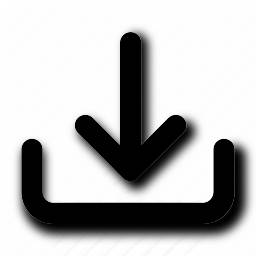
\includegraphics[width=5.5mm]{pictures/white_bk/upload.png}, which is right beside the Operating System Selector popup on the toolbar.

You can upload as many files (.dd) as you want. But only run one at a time.

In duckyscript, it is normally not possible to write a program that uses multiple files at a time, except it is possible in a USB Pico Ducky. You can also switch between the payloads using the white switch on the USB Pico Ducky.

This is useful for when you need different payloads for different OSs. For example, you might want to have a Mac version and a Windows version of a password brute-forcing payload. This is useful for when you aren't sure about the OS of the target computer. \textbf{Not even USB Rubber Ducky comes with this feature}

\textbf{The valid payload names are: payload.dd, payload1.dd\dots}

\subsection{Execute}

\subsubsection{Before Execution}

Before Execution, first select the target device's OS, then language (in order). Currently Mac supports less languages then Windows does, therefore make sure to select device's OS first

\subsubsection{Run Duckyscript Program}

To Execute a duckyscript program, insert the USB into a device while in attack mode. Turn on hack mode as specified in section \ref{hack_mode_on}

\subsubsection{Run C/C++/Python Program}

To run a C/C++/Python (or any supported language) program. Please refer to section \ref{hack_mode_off} to setup the microcontroller.

Since the USB Pico Ducky is a Raspberry Pi Pico MicroController, you can run a C/C++/Python program as you wish as long as the hacking mode is turned off. Please note that the IDE doesn't support these languages. Therefore use a different IDE or text editor of your choosing. The IDE only supports duckyscript.

\section{Duckyscript Language}

Duckyscript language is a language used in hacking USBs. Hacking USBs pretend to be Perhipheral devices such as keyboards. Duckyscript is a simple language that is used in certain microcontrollers to mimic keyboards.

\subsection{Keywords}\label{all_keywords}

All the keywords:

Here are some keyboard keys supported by All languages
\scriptsize
$\\\begin{bmatrix} 
REM & DELAY & STRING & PRINT & DEFAULT\_DELAY
\\DEFAULTDELAY & LED & REPEAT & IMPORT & ENTER
\\F1-F12 & ALT & CTRL & CONTROL & SHIFT & SPACE
\\BACKSPACE & ESC & ESCAPE & UP & UPARROW & DOWN
\\DOWNARROW & LEFT & LEFTARROW & RIGHT & RIGHTARROW
\\WINDOWS & GUI & A-Z & APP & MENU
\\DELETE & END & HOME & INSERT & NUMLOCK & PAGEUP
\\PAGEDOWN & PRINTSCREEN & SCROLLLOCK & BREAK & PAUSE
\end{bmatrix}\\\\$
\normalsize

Some of these keywords are the same keyboard key, this website shows which keywords share the same meanings
https://wiki.spacehuhn.com/wifiduck/usage/duckyscript/

\subsection{Tutorial}

As you can see on section \ref{all_keywords}, all these keywords have to be capital. If you type it correctly, the keyword will change color on the IDE (only if it's used at the beginning of a line), this way you can now that you typed it correctly.

as you can see most of these keywords can be found on the keyboard. This is because everything else is just keyboard keys and the function of these keys depend on the OS (Operating System), the type and brand of the device. 

\begin{center}
\setlength{\arrayrulewidth}{0.3mm}\begin{tabular}{|b|b|}
	\cline{1-2}
	\multicolumn{2}{|r|}{Here are the duckyscript commands that aren't keyboard keys}\\
	\centering\setlength{\extrarowheight}{7pt}
	REM & Stands for 'REMOVE', it's used for commenting code\\
	\hline
	DELAY & \thead{A pause (in milliseconds). Used for when waiting for\\ an interface to catch up with \\ the USB Pico Ducky typing speed}\\
	\hline
	STRING & \thead{Types whatever comes after the command}\\
	\hline
	REPEAT & \thead{Repeats the previous command N times}\\
	\hline
	PRINT & \thead{Prints whatever comes after to python console}\\
	\hline
	IMPORT & \thead{Imports and executes another duckyscript file to execute\\(has to be in the same path/folder), this functionality doesn't exist in the\\USB Rubber Ducky but does exist in this USB Pico Ducky.}\\
	\hline
	\thead{DEFAULTDELAY \\DEFAULT\_DELAY} & \thead{Specifies how long (in milliseconds) to\\wait between each line of command. If not specified, DEFAULTDELAY is 18ms.}\\
	\hline
	LED & \thead{Change the state of the LED (on/off)}\\
\end{tabular}
\end{center}

\begin{center}
\begin{tabular}{|b|g|}
	\multicolumn{2}{|r|}{Keys That Might Be Confusing}\\
	\hline
	WINDOWS \& GUI & The windows button\\
	\hline
	UP \& UPARROW & The up arrow key\\
	\hline
	DOWN \& DOWNARROW & The down arrow key\\
	\hline
	RIGHT \& RIGHTARROW & The right arrow key\\
	\hline
	LEFT \& LEFTARROW & The left arrow key\\
	\hline
\end{tabular}
\end{center}

All the rest of the keywords can be found on a keyboard\\

Keyboard keys are used for typing and shortcuts that are OS (Operating System) dependant. For example, F-keys (e.g. F1 key) won't work on a phone because there is no such thing as F1 button on a phone, also the function of keys change depending on the OS (Operating System).

Payload examples can be found in section \ref{duckyscript_examples}.

\subsection{Examples}\label{duckyscript_examples}

\subsubsection{Comment (REM)}

\begin{figure}[htb]
\begin{small}
\begin{lstlisting}[language=Ducky]
REM this is a comment
\end{lstlisting}
\end{small}
\caption{Comment Example}
\end{figure}

This code shows an example on how to comment, note that REM is one line comment. The USB Pico Ducky only supports Duckyscript 1.0 which doesn't have Multi-line comments.

\subsubsection{DELAY}

\begin{figure}[htb]
\begin{small}
\begin{lstlisting}[language=Ducky]
REM delay by 500 miliseconds before locking windows pc (opens lockscreen)
DELAY 500
WINDOWS L
REM in the code above, windows takes the L (like always, nearly all viruses and attacks target windows)
\end{lstlisting}
\end{small}
\caption{Delay Example}
\end{figure}

In the code above, the payload is delayed by 500ms (delayed so that the device is ready to type). the WINDOWS+L Button is pressed which is the shortcut to the lockscreen on windows

\newpage

\subsubsection{STRING}

\begin{figure}[htb]
\begin{small}
\begin{lstlisting}[language=Ducky]
REM delay by 100 miliseconds before starting a windows powershell
DELAY 100
GUI R
STRING powershell
ENTER
\end{lstlisting}
\end{small}
\caption{STRING Example}
\end{figure}

This code delays by a 100ms, presses WINDOWS+R Shortcut, types in powershell, presses enter button.

\subsubsection{REPEAT}

\begin{figure}[htb]
\begin{small}
\begin{lstlisting}[language=Ducky]
REM delay by 100 miliseconds before starting 10 new google tabs
DELAY 100
WINDOWS S
STRING chrome
ENTER
CTRL T
REPEAT 10
\end{lstlisting}
\end{small}
\caption{REPEAT Example}
\end{figure}

In this code, there is an initial delay of 100ms when the execution starts, then the WINDOWS+S button is pressed which opens search bar, enters chrome, presses enter, than types CTRL+T (new google tab), repeats the last command 10 times. It basically presses CTRL+T 10 times which opens 10 tabs

\newpage

\subsubsection{PRINT}

\begin{figure}[htb]
\begin{small}
\begin{lstlisting}[language=Ducky]
REM delays by 300 miliseconds, and opens 10 google tabs, then prints successfully opened 10 tabs
DELAY 300
WINDOWS S
STRING chrome
ENTER
CTRL T
REPEAT 10
PRINT Successfully opened 10 tabs
\end{lstlisting}
\end{small}
\caption{PRINT Example}
\end{figure}

In this code, there is an initial delay of 100ms when the execution starts, then the WINDOWS+S button is pressed which opens search bar, enters google, presses enter, than types CTRL+T (new google tab), repeats the last command 10 times. It basically presses CTRL+T 10 times which opens 10 tabs. Then once it's done, it types Successfully opened 10 tabs to a python console.

\newpage

\subsubsection{IMPORT}\label{ducky_import}
For example, there are 2 files, payload.dd and payload2.dd (there can be as many as you wish)
\begin{figure}[htb]
\begin{small}
\begin{lstlisting}[language=Ducky]
REM delay by 300ms, then paste the last copied thing onto a notepad
DELAY 300
WINDOWS R
STRING notepad.exe
ENTER
CTRL V
PRINT Successfully printed the last thing that was copied onto a notepad
\end{lstlisting}
\end{small}
\caption{payload.dd}\label{import_1}
\end{figure}

\begin{figure}[htb]
\begin{small}
\begin{lstlisting}[language=Ducky]
REM wait 500ms, import payload.dd (import keyword executes the file specified)
DELAY 500
IMPORT payload.dd

REM save file and close all notepad files
DELAY 100
CTRL S
CTRL SHIFT W
\end{lstlisting}
\end{small}
\caption{payload2.dd}\label{import_2}
\end{figure}

in figure \ref{import_1}, there is an initial delay of 300 miliseconds, then presses WINDOWS+R (opens run box), then types notepad.exe, presses enter. Now that notepad is opened, presses CTRL V (types the last copied thing in the clipboard), then prints that it 'successfully printed the last copied thing onto a notepad' into a python console.

in figure \ref{import_2}, there is an initial delay of 500ms, then imports and executes the content of payload.dd. Then, delays by 100ms, presses CTRL+S (save) and CTRL+SHIFT+W (exit)

\newpage

\subsubsection{DEFAULTDELAY \& DEFAULT\_DELAY}

\begin{figure}[htb]
\begin{small}
\begin{lstlisting}[language=Ducky]
REM set default delay to 250, this will cause all commands being executed once every 250ms
DEFAULTDELAY 100
WINDOWS R
STRING notepad.exe
ENTER
STRING Every command is being executed after a delay of 250ms
\end{lstlisting}
\end{small}
\caption{DEFAULTDELAY Example}\label{defaultdelay_example}
\end{figure}

in the code above (figure \ref{defaultdelay_example}), there is no initial delay, but the default delay is moved to 100ms, which means that every command will delay by 100ms before execution(so that the device can catch up), then presses WINDOWS+R (opens run box), then type notepad.exe, presses enter.

Note that the default delay only applies to one file. Therefore if you import a different file, the custom default\_delay won't apply to the imported file

\subsubsection{LED}

\begin{figure}[htb]
\begin{small}
\begin{lstlisting}[language=Ducky]
REM wait 500ms, then update LED status once successfully installed mimikatz virus from the web
DELAY 500
WINDOWS S
STRING chrome
ENTER
STRING https://github.com/gentilkiwi/mimikatz/releases/download/2.2.0-20220919/mimikatz_trunk.zip
ENTER
DELAY 300

REM once the virus downloads, turn on the LED of USB Pico Ducky
LED
\end{lstlisting}
\end{small}
\caption{LED Example}\label{led_example}
\end{figure}

in the code above (figure \ref{led_example}), there is an initial delay of 500ms. Then the WINDOWS+L button is pressed (run box), chrome is typed into the run box, then ENTER is pressed. Now that google chorme is open, this link is opened: \nolinkurl{https://github.com/gentilkiwi/mimikatz/releases/download/2.2.0-20220919/mimikatz_trunk.zip} which downloads the zip file of the mimikatz virus.

\newpage

\section{Setup}

\subsection{Reset}

\subsubsection{When to Reset USB}

Resetting the USB turns hacking mode off. More information can be found in section \ref{hack_mode_off}. You can also reset back to the USB Pico Ducky (hacking mode) as specified in more detail in section \ref{hack_mode_on}.

\subsubsection{How to Reset USB}\label{how_to_reset}

You can reset the USB at any time, all it takes is the click of a simple button in the Duckyscript IDE (on the toolbar). The button is 
\includegraphics[width=5.5mm]{pictures/setup.png}. This button is at the most right on the toolbar. After clicking this button, a popup window will come up. Click the button on the middle (Select USB Pico Ducky Path), then select the path of your USB pico ducky. Now Another button will popup, if you entered the correct path, select the new button (Enable/Disable hacking mode) on the popup.

\subsection{Hack Mode On}\label{hack_mode_on}

\subsection{Hack Mode Off}\label{hack_mode_off}

When the USB Pico Ducky hack mode is turned off, you can use the microcontroller using C/C++/MicroPython (resources in section \ref{cc_lang}).


\subsubsection{C/C++/MicroPython Language}\label{cc_lang}

Here are some helpful links on setting up C/C++/Python for a Raspberry Pi Pico

\textbf{Windows Tutorials:}\\
\indent\indent 1. \underline{\href{https://www.raspberrypi.com/news/raspberry-pi-pico-windows-installer/}{C Language}}

\indent\indent 2. \underline{\href{https://www.raspberrypi.com/news/raspberry-pi-pico-windows-installer/}{C++ Language}}

\indent\indent 3. \underline{\href{https://how2electronics.com/raspberry-pi-pico-getting-started-tutorial-with-micropython/}{MicroPython Langauge}}\\

\textbf{Mac/Linux Tutorials:}

\indent\indent 1. C Language:
\begin{description}
	\setlength{\itemindent}{3em}
	\item[$\bullet$] \underline{\href{https://www.electronicshub.org/program-raspberry-pi-pico-using-c/}{Tutorial in Linux}}
	\item[$\bullet$] \underline{\href{https://blog.smittytone.net/2021/02/02/program-raspberry-pi-pico-c-mac/}{Tutorial in Mac}}
\end{description}

\indent\indent 2. C++ Language:
\begin{description}
	\setlength{\itemindent}{3em}
	\item[$\bullet$]\underline{\href{https://circuitdigest.com/microcontroller-projects/how-to-program-raspberry-pi-pico-using-c}{Tutorial in Linux}}
	\item[$\bullet$]\underline{\href{https://www.peterzimon.com/raspberry-pi-pico-mac-c-getting-started/}{Tutorial in Mac}}
\end{description}

\indent\indent 3. MicroPython Language:
\begin{description}
	\setlength{\itemindent}{3em}
	\item[$\bullet$]\underline{\href{https://circuitdigest.com/microcontroller-projects/getting-started-with-raspberry-pi-pico-with-micropython}{Tutorial in Linux}}
	\item[$\bullet$]\underline{\href{https://desertbot.io/blog/raspberry-pi-pico-setup-mac}{Tutorial in Mac}}
\end{description}

\large
\emph{\textbf{Other Helpful Sources:}}
\normalsize
\begin{description}
	\setlength{\itemindent}{3em}
	\item[$\bullet$] \underline{\href{https://how2electronics.com/raspberry-pi-pico-getting-started-tutorial-with-micropython/}{MicroPython Tutorial}}
	\item[$\bullet$] \underline{\href{https://www.raspberrypi.com/documentation/microcontrollers/c_sdk.html}{Raspberry Pi Pico Documentation for C/C++}}
\end{description}

\subsubsection{Upload}

The Duckyscript IDE doesn't have C/C++ support at this time. To use C/C++ on the USB Pico Ducky. First, reset the USB as mentioned in section \ref{how_to_reset}, then use a different IDE/texteditor to write a C/C++ program. You can reserach for more information in section \ref{cc_lang}.

\newpage

\end{document}
